We gebruiken bovenstaande code om $sin(x)$ en $\frac{1}{1+7x^2}$ te benaderen op het interval [-2,2] met een equidistante set van 10 abscissen voor $sin(x)$ en 9 abscissen voor de tweede functie. We vergelijken dit ook met een veelterminterpolant door deze punten. Het eerste resultaat is te vinden in figuur \ref{fig:sinequi}, het tweede resultaat in figuur \ref{fig:ratequi}. We geven steeds een plot van de functiewaarden en van het residu weer.
\\
De functie $\frac{1}{1+7x^2}$ is een klassiek voorbeeld van een functie die slecht te banderen is met een interpolerende veelterm door equidistante punten. Dit is duidelijk te zien in de plot van het residu. De splinevoorstelling presteert hier een stuk beter. 
\\
TODO verdere uitleg over verschil veelterm vs. spline bij sin??

\begin{figure}
\centering
\begin{subfigure}{.5\textwidth}
  \centering
  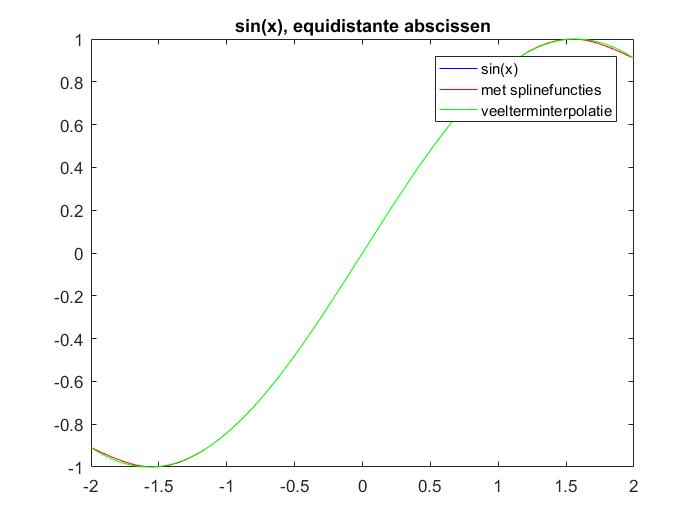
\includegraphics[width=\linewidth]{afbeeldingen/sin_equi.jpg}
  \caption{functiewaarden}
\end{subfigure}%
\begin{subfigure}{.5\textwidth}
  \centering
  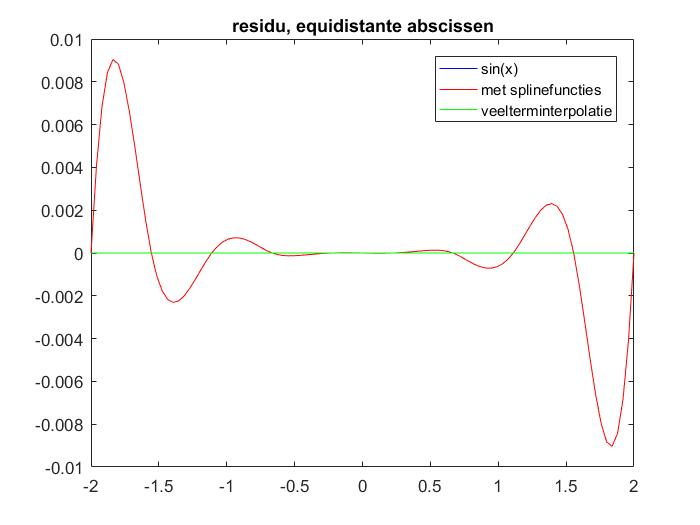
\includegraphics[width=\linewidth]{afbeeldingen/sin_equi_res.jpg}
  \caption{residu}
\end{subfigure}
\caption{interpolant door 10 equidistante absciswaarden van $sin(x)$}
\label{fig:sinequi}
\end{figure}

\begin{figure}
\centering
\begin{subfigure}{.5\textwidth}
  \centering
  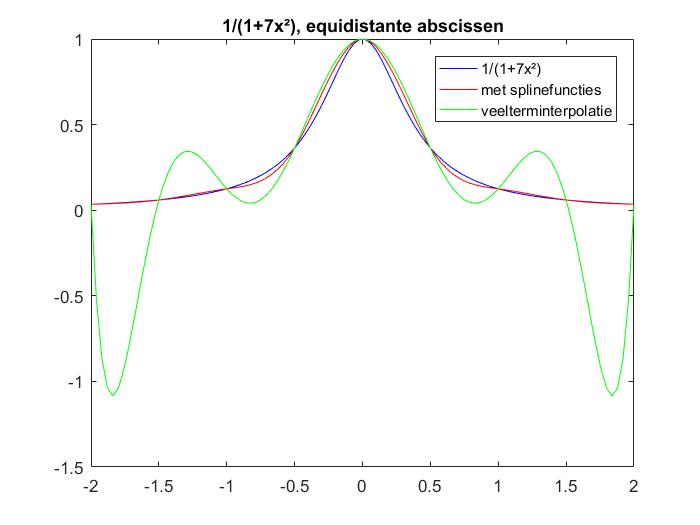
\includegraphics[width=\linewidth]{afbeeldingen/rat_equi.jpg}
  \caption{functiewaarden}
\end{subfigure}%
\begin{subfigure}{.5\textwidth}
  \centering
  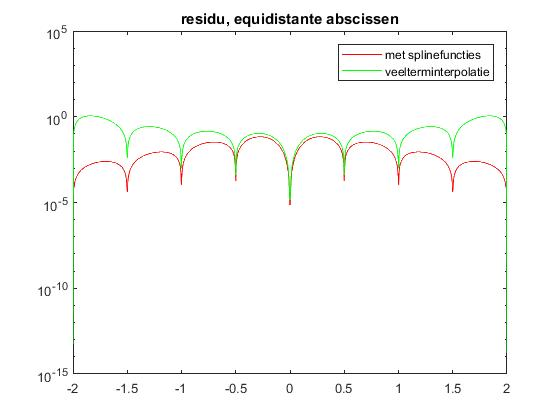
\includegraphics[width=\linewidth]{afbeeldingen/rat_equi_res.jpg}
  \caption{residu}
\end{subfigure}
\caption{interpolant door 9 equidistante absciswaarden van $\frac{1}{1+7x^2}$}
\label{fig:ratequi}
\end{figure}